%location/filename: tex/ch1.tex
%author: Anders Østevik
% Created: 28.2.2016
%#######--Chapter 4--#######
%Content:	

\documentclass[main.tex]{subfiles}

%\usetikzlibrary{arrows,automata}

\begin{document}

\chapter{External and Internal Loopback Test of the GBT Bank Quartus Example}

\section{120 MHz Reference Clock}

%\todo{name the proper plls and state why 120 mhz is really needed} 

To be able to conduct a proper loopback test, the \gls{mgt} and the \glspl{pll} of the \gls{gbt} must have a input clock frequency of $120~\mega\hertz$. There are a number of ways to achieve this on the Cyclone V board: 
\begin{itemize}\setlength{\itemsep}{10pt}
\item Using an external clock, like a square wave signal generator.
\item Using one of the on-board programmable oscillators.
\item Implementing a \gls{pll} into the design that multiplies the on-board $50~\mega\hertz$ global clock up to the desired frequency of $120~\mega\hertz$.
\end{itemize}

The original approach is to use an external signal generator with differential output to generate the reference clock, as shown in the \gls{gbt} tutorial videos \cite{gbt_videos}. However, at the time of conducting the first tests, there was no available signal generators that could generate a $120~\mega\hertz$ square wave clock for the experiment. Because of this, some time was spent to investigate how to use the internal programmable oscillator as a reference clock.\\

The approach of implementing an extra \gls{pll} into the \gls{gbt}-example design was also investigated, but attempts of doing so resulted in conflicts between the already implemented transceiver \glspl{pll} in the design. \\

The below sections gives the following descriptions:
\begin{itemize}\setlength{\itemsep}{10pt}
\item How to setup the internal oscillator on the Cyclone V board for use as reference clock.
\item How to setup the $Si338$ external oscillator for use as reference clock.
\end{itemize}

\section{Configuring the On-board Oscillator on the Cyclone V Board}

To achieve a reference clock of $120~\mega\hertz$ without an external clock, the \gls{fpga} has an on-board programmable oscillator; the $Si570$ from Silabs. It uses \gls{iic} for serial communication and can be programmed to output frequencies up to $810~\mega\hertz \pm 50 ppm$. To program the oscillator, Altera provides a dedicated software called "Clock Control". The Clock Control software is part of the Java based "Board Test System" software, included in the Cyclone V kit which can be found at Altera's websites \cite{altera_cyclonekit}. The Cyclone V kit is board specific, so it is therefore important to use the right kit with the right board.\\

To make use of the Clock Control software has been proven difficult, mainly because of the software being outdated in relevance to the current version of Quartus (at the time of writing, Quartus 15.0 is the newest edition). The solution was to install an older Quartus (version 13.1) using the Windows Operating System (Linux was also attempted, but without any success) and specify the right paths for the related environment variables. The below sections gives a brief description on how this was achieved.\\

\subsection{Clock Control Software Setup}

The Cyclone V kit is dependent on a number of Quartus related files, including the USB Blaster II device driver, the jtagconfig software and various device libraries included in the Quartus environment. It is therefore important to have the right version of Quartus installed for the Clock Control program to work properly. The version number of the kit (13.0.0.1 at the time of writing) corresponds to the supported version of Quartus, in this case Quartus 13.x (newer versions of Quartus have not proven to be backwards compatible with the Cyclone V kit).\\

By using Windows, the following steps have been proven to be the best approach to make the Clock Control software work properly. The installed path to Quartus is in this case: \path{D:\Quartus_13.1}.\\

\subsection{Steps for Configuring Windows to run the Clock Control Software}

\begin{enumerate}\setlength{\itemsep}{10pt}
  \item Install Quartus 13.x (includes jtagconfig) together with the Cyclone V device support \cite{altera_q13}.
  \item Set appropriate environment variables. In Windows, this should be set automatically.
  \begin{itemize}\setlength{\itemsep}{10pt}
      \item PATH -- \path{"D:\Quartus_13.1"}
      \item QUARTUS\_ROOTDIR -- \path{"D:\Quartus_13.1\quartus"}
      \item SOPC\_KIT\_NIOS2 -- \path{"D:\Quartus_13.1\nios2eds"}
    \end{itemize}
  \item Connect the Cyclone V board to the \gls{pc} using USB Blaster II (Refer to the manual for instructions on how to install the USB Blaster II \cite{altera_usb}).
  \item In Command Prompt (cmd.exe):
  \begin{itemize}\setlength{\itemsep}{10pt}
      \item Navigate to the "board\_test\_system" folder located inside the Cyclone V kit.
      \item run "jtagconfig" and confirm connection with the board. If the Command Prompt cannot find jtagconfig, navigate to \path{D:\Quartus_13.1\quartus\bin} using a file explorer and manually start jtagconfig.exe from there
      \item run "java -Djava.library.path=\path{"D:\Quartus\_13.1\bin"} -jar clk\_cont.jar". The library path is to ensure that the Java environment have access to the appropriate Quartus libraries it needs to connect with the board.
    \end{itemize}
\end{enumerate}

If done correctly, the Clock Control software will start up and display "Connected to the target" in the message window. The default output frequency of the $Si570$ oscillator is $100~\mega\hertz$. The output frequency is calculated using the following equation:

\begin{equation}
%\[
    f_{out} = \frac{f_{XTAL} \times RFREQ}{HSDIV \times N1}
%\]
\end{equation} 

, where $f_{XTAL}$ is a fixed frequency of $114,2857~\mega\hertz$; RFREQ is a floating point 38-bit word; and HSDIV and N1 is the output dividers \cite{si570}. The parameters are determined by the Clock Control software based on the user typed frequency. The parameters are then sent serially via the USB Blaster II to the $Si570$ chip, where the above formula is used to set the internal registers for the new frequency.
Figure \ref{fig:clk_cont120} shows the Clock Control software after a new frequency of $120~\mega\hertz$ is set. 

\begin{figure}[] % H(strictly put HERE > h!)
\begin{center}
% h(here), !(force), t(top), b(bottom), p(on extra page)
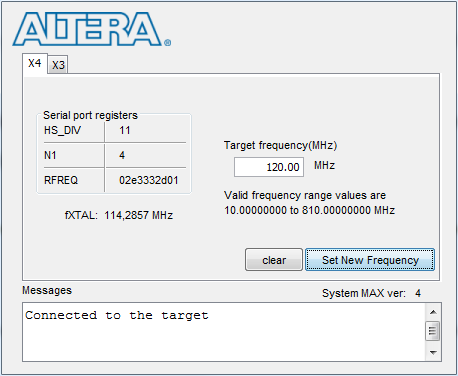
\includegraphics[scale=1]{../img/clk_cont120}  \\[0.1 cm]
\caption{Clock Control software by Altera used to program the $Si570$.}
\label{fig:clk_cont120}
\end{center}
\end{figure} 

The $Si570$ is volatile, meaning that the output frequency is reset back to $100~\mega\hertz$ if power is lost. The procedure must therefore be repeated every time the \gls{fpga} is powered on.\\
To confirm correct operation, a quick measurement of the output clock was done using an oscilloscope. Figures \ref{fig:tek100} and \ref{fig:tek120} shows the output frequency, before and after configuration.\\

\begin{figure}[]
   \begin{floatrow}
     \ffigbox{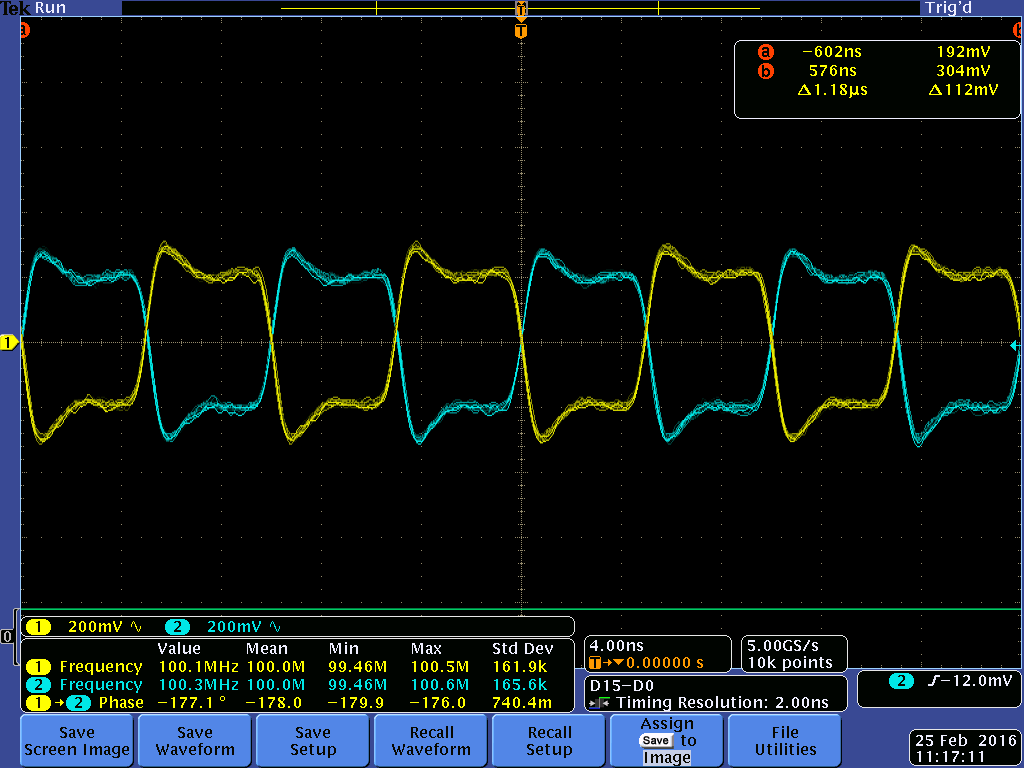
\includegraphics[scale = 0.2]{../img/20160226_tek100}}{\caption{$Si570$ Before configuration: 100 MHz.}\label{fig:tek100}}
     \ffigbox{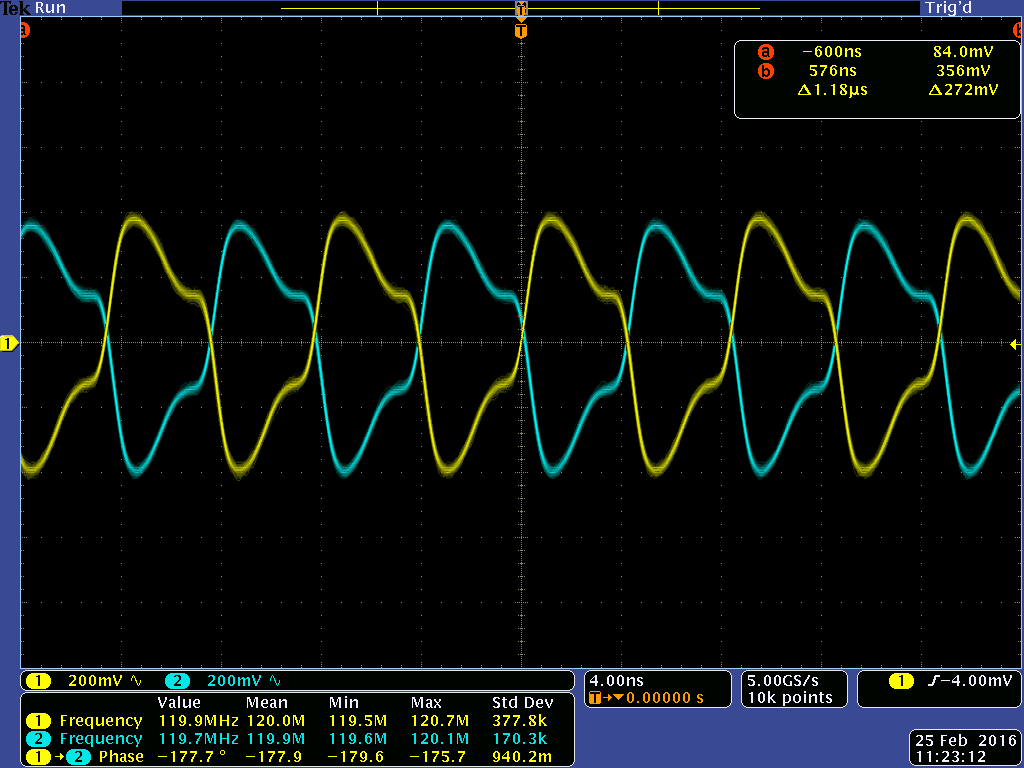
\includegraphics[scale = 0.2]{../img/20160226_tek120}}{\caption{$Si570$ After configuration: 120 MHz.}\label{fig:tek120}}
   \end{floatrow}
\end{figure}

\section{Configuring the $Si338$ External Oscillator}


\chapter{Testing and Verification of the HDMI Daughter Card}
To verify a working \gls{pcb}, the \gls{hdmi} daughter card underwent a series of tests. The sections below summarizes these tests. 

\section{Connectivity Test}

\textit{Since all the components on the \gls{pcb} was hand soldered (with the exception of the ground pads underneath the \gls{hsmc} contact), it was particularly important to check for accidental shorts between pins and/or pads.}

\subsection{Purpose of Test}

\begin{itemize}\setlength{\itemsep}{10pt}
\item Verify that there are no shorts between the pins and/or pads of the \gls{pcb}. 
\item Check for current draw to confirm that there are no short on the power-lines.
\end{itemize}

\subsection{Experimental Setup}

The setup involves the use of a multimeter to go through all pins and check for connection faults according to the schematic. After all shorts have been eliminated, the \gls{pcb} is to be connected to an external power supply to verify current-draw. 

\subsection{Results}
 Using a multimeter, all connections were checked and verified that there were no shorts (Some pins on the \gls{hsmc} were indeed shorted and had to be re-soldered). The \gls{pcb} was then connected to an external power supply, with a $3.3~\volt$ output and a current output limited to $100~\milli\ampere$. It was verified that the current draw, with all \gls{hdmi}-connections left open, were no more than the current drawn from the power-\acrshort{led} and the $1.25~\volt$ voltage divider, i.e around $40~\milli\ampere$. \\

To confirm connectivity and that there were no further connecting shorts between the pads and/or pins, a simple test-circuit was written in Quartus. Beginning with the transmit-signals: all the relevant \gls{lvds} transmit-signals that are physically connected to the \gls{hsmc} (port A) connector of the \gls{fpga} were connected to a given clock signal. The \gls{pcb} was then connected to the Cyclone V board, and the \gls{hdmi} connectors were probed with the help of an oscilloscope and verified that there was an output signal on every \gls{hdmi}-transmitter. 

The \gls{pcb} is now ready for connection with the host \gls{fpga} for further testing of the transmitter and receiver signals. 

\section{External Loop-back Test for the Fiber-Optic Connector} \label{sec:exlooptest}

\textit{To verify that the \gls{hdmi} daughter card SFP-connector for fiber-optic communication is working correctly, an external loop-back test was conducted.}

\subsection{Purpose of Test}
\begin{itemize}\setlength{\itemsep}{10pt}

\item Test the dedicated SFP-connector on the \gls{hdmi}-daughter card for fiber-optic communication and see that it is capable of sending and receiving information at speeds corresponding the \gls{gbt}-standard of $4.8 \giga\bit\per\second$. 
\end{itemize}

\subsection{Experimental Setup}
A fiber-optic cable connected from the transmitter to the receiver using a fiber-module, forming an external loop through the cable, was connected to the SFP-connector of the \gls{hdmi}-daughter card \gls{pcb}. Using the \gls{gbt} Quartus-example together with the \gls{issp} and SignalTap II, it was possible to perform a pattern check test by comparing the transmitted signals with the received signals. To achieve this test, \gls{issp} was used to setup the pattern generator of the GBT example to count with increments of one (PATTERN SELECT = "1h") and the receiver to receive signals through external cabling (LOOPBACK = '0'). SignalTap II was used to monitor and verify that the receiver line received the same incremented counter that the transmitter sent out.

\subsection{Results}
Running the test resulted in a continuous stream of bits sent from the transmitter to the receiver. Using SignalTap II as a monitor limits to only observe parts of the transmission, but it was sufficient enough to see that the received sum of bits were indeed incrementing by one each time, and with this conclude that the SFP-connector on the HDMI-daughter card works as intended at $4.8 \giga\bit\per\second$. Figure \ref{fig:lb_rx} shows the resulting incremented sum of bits transmitted and received at the receiving end.


\section{External Loop-back Test for the HDMI Connectors}

\subsection{Purpose of Tests}

\begin{itemize}\setlength{\itemsep}{10pt}
\item Measure the quality of the signal (eye-diagram) at different frequencies up to $300~\mega\hertz$ and see how reflections affects the signal.
\item Measure crosstalk between neighboring signal paths.
\item Create a test environment using Quartus II in conjunction with SignalTap II to:
\begin{itemize}\setlength{\itemsep}{10pt}
  \item See if it is possible to sample the received signals at different frequencies up to $300~\mega\hertz$.
  \item Calculate the bit-error rate at different frequencies up to $300~\mega\hertz$.
\end{itemize}
\end{itemize}

\subsection{Experimental Setup}

Each \gls{hdmi}-connector has at least one transmitter- and receiver line. To simulate signal transmission over a distance, a \gls{hdmi} cable was cut in half and the transmit- and receive lines were soldered together, creating an external loop-back. A pseudo-random generated bit-signal would travel out via one of the transmitters of the \gls{fpga}, out through a \gls{hdmi}-connector, following the cable back into the same \gls{hdmi}-connector into the receiver input. This is to simulate the transmission path to the \gls{vldb} card. Because of the trace- and cable-length, a delay is introduced between the transmitted and received signal. As mentioned in chapter \ref{chap:pcb}, a signal propagates through the conductor at a velocity of approximately $15\ \milli\meter/\nano\second$. Cables with two different lengths were tested, to see if it would affect the bit-error rate.

To measure the quality of the \gls{lvds} signals with an oscilloscope, differential probes were used.  


\subsection{Results}

%The following table sums up the cable-length and theoretical travel time versus the measured delay between the transmitted and received signal.

\section{Conclusion and Discussions}


When measuring the quality of a high-speed signal, the way you measure the signal can have a major impact on the result. This was experienced when attempting to measure the \gls{lvds} signals using the differential probes. On the first attempt, small clamps connected to each of the differential probes (figure \ref{fig:hektere}) were coupled to a differential pair that were running from one end of a hdmi-cable, with a terminating resistor in between; in to a transmitter on the \gls{hdmi}-daughter card. A clock signal was sent from the \gls{fpga} throught the \gls{hdmi}-daughter card to the end of the hdmi-cable. 

\begin{figure}[H] 
   \begin{center}
     \ffigbox{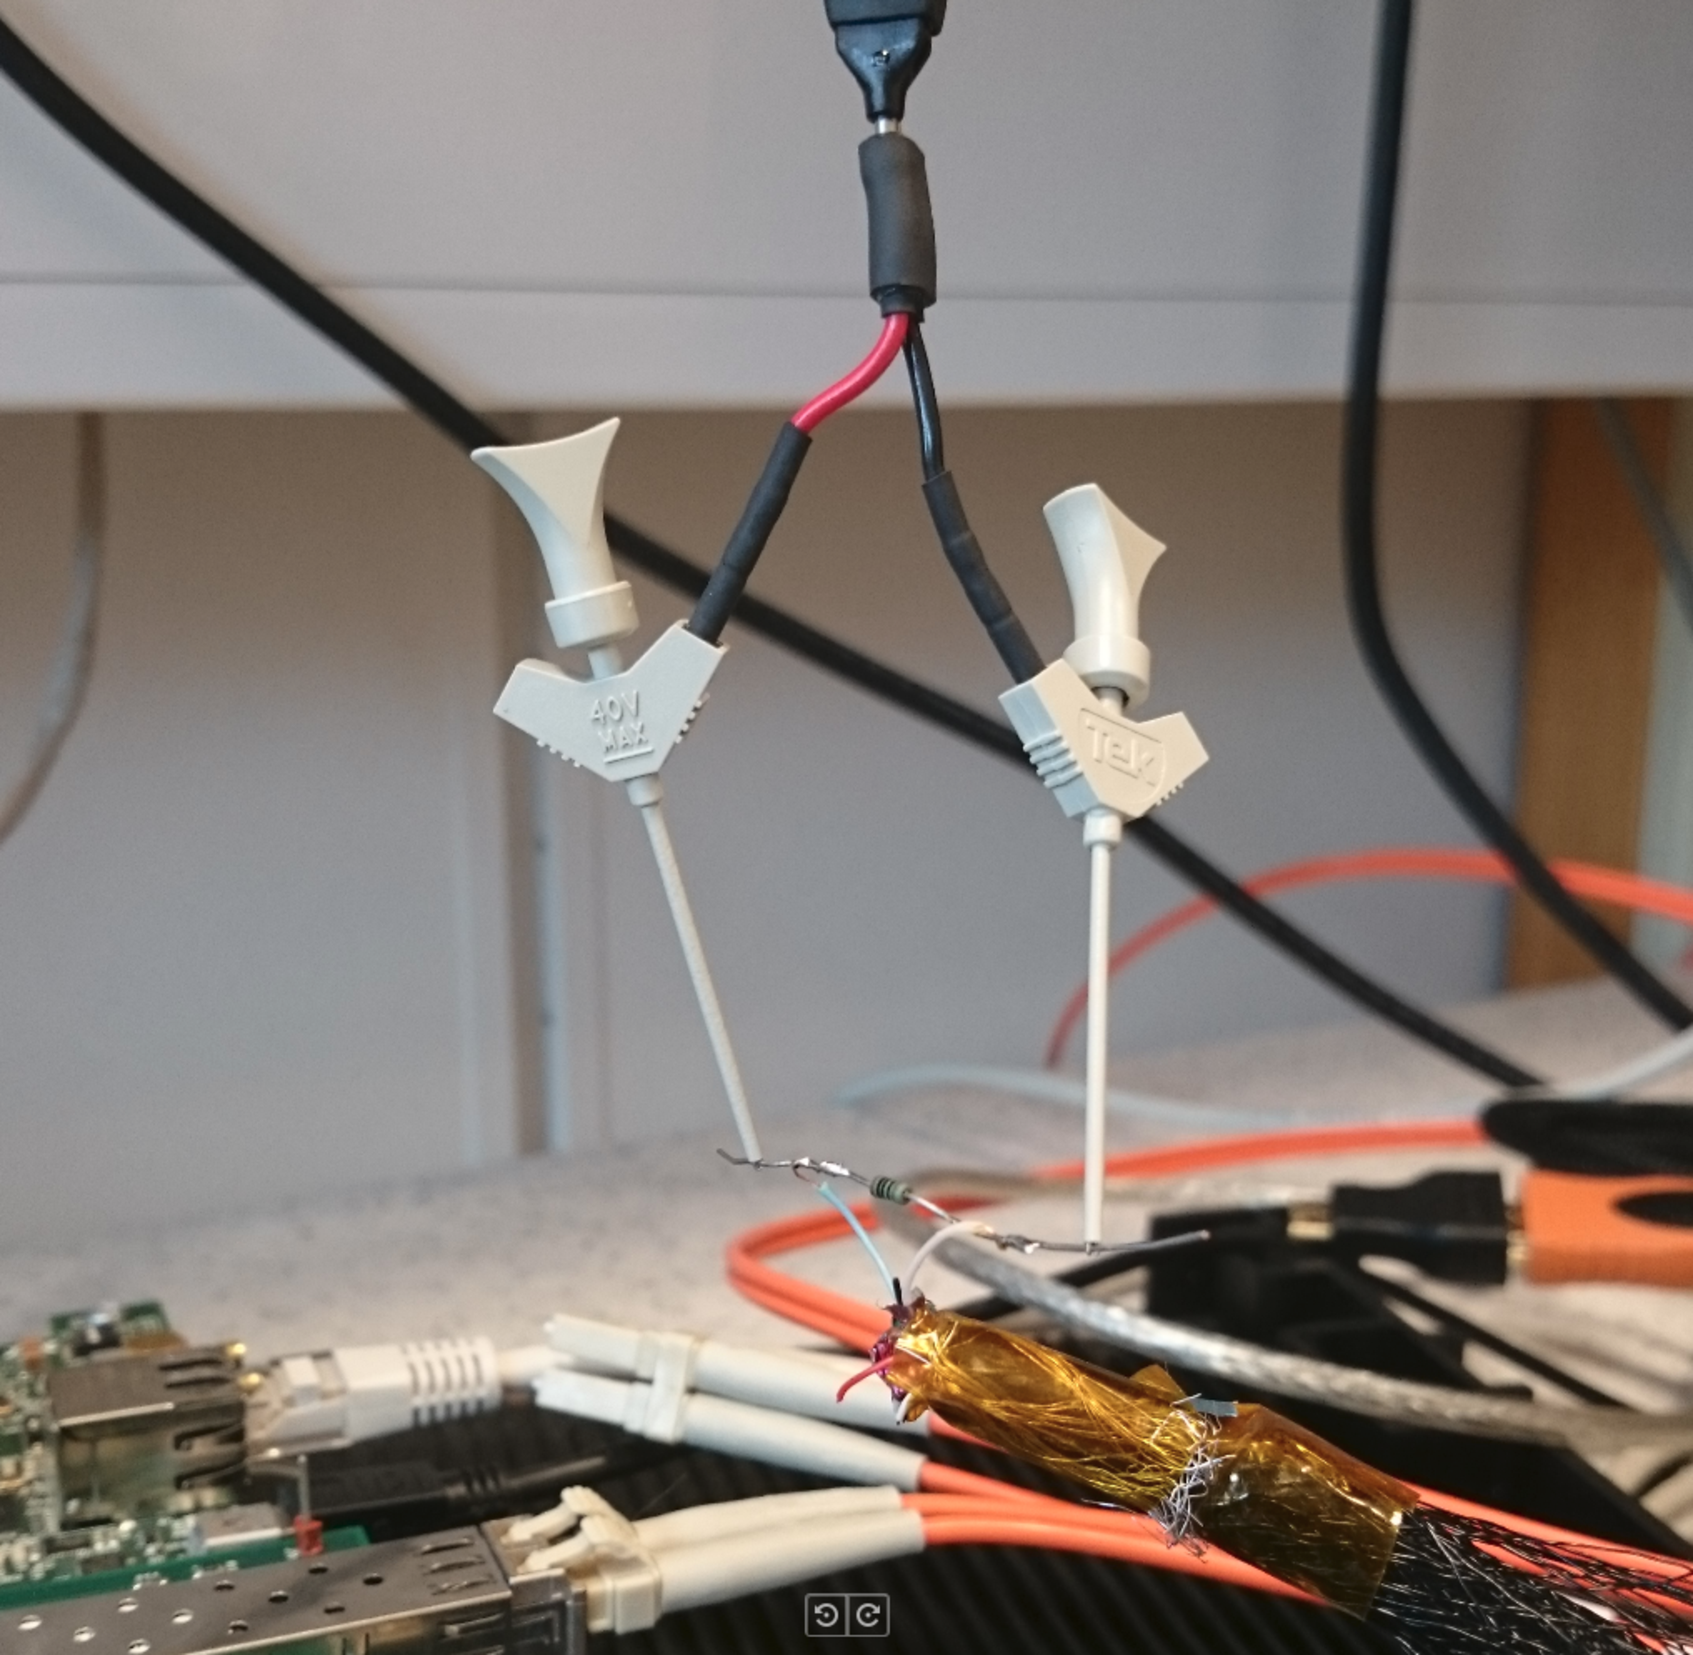
\includegraphics[scale = 0.2]{../img/hektere_probes.pdf}}{\caption{Small clamps was first used to measure the high-speed signal.}\label{fig:hektere}}
   \end{center}
\end{figure}

The measurement resulted in signals that were heavily distorted by reflections. It was first thought that these reflections might originate from the traces on the \gls{fpga} itself, since the same results were produced when sending the clock signals through a different \gls{pcb} (a GPIO-card) in place of the \gls{hdmi}-daughter card. However, the theory was quickly rejected when using a completely different \gls{fpga} board produced the same reflections. The cause was in fact due to the small clamps that was used to connect the differential probes. By replacing these with small stubs and redo the measure, the result was quite different, as shown in figures \ref{fig:measdiff1} and \ref{fig:measdiff2}.

\begin{figure}[H]
   \begin{floatrow}
     \ffigbox{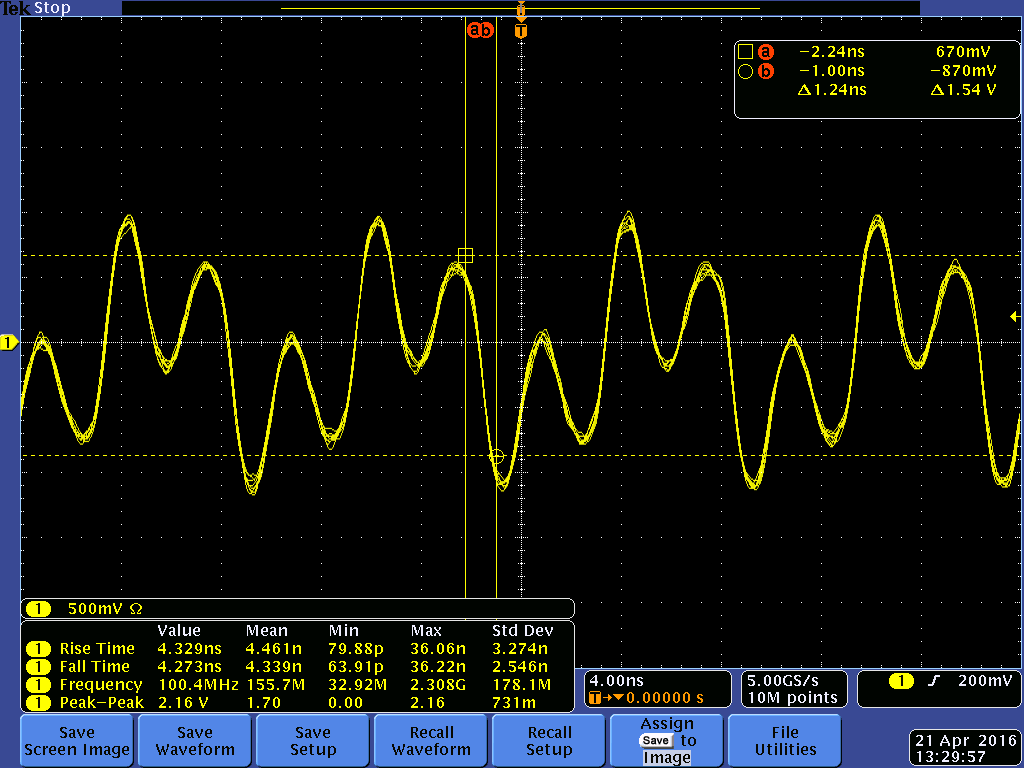
\includegraphics[scale = 0.2]{../img/hektere_oppsett_100mhz.png}}{\caption{$100~\mega\hertz$ measured using clamps.}\label{fig:measdiff1}}
     \ffigbox{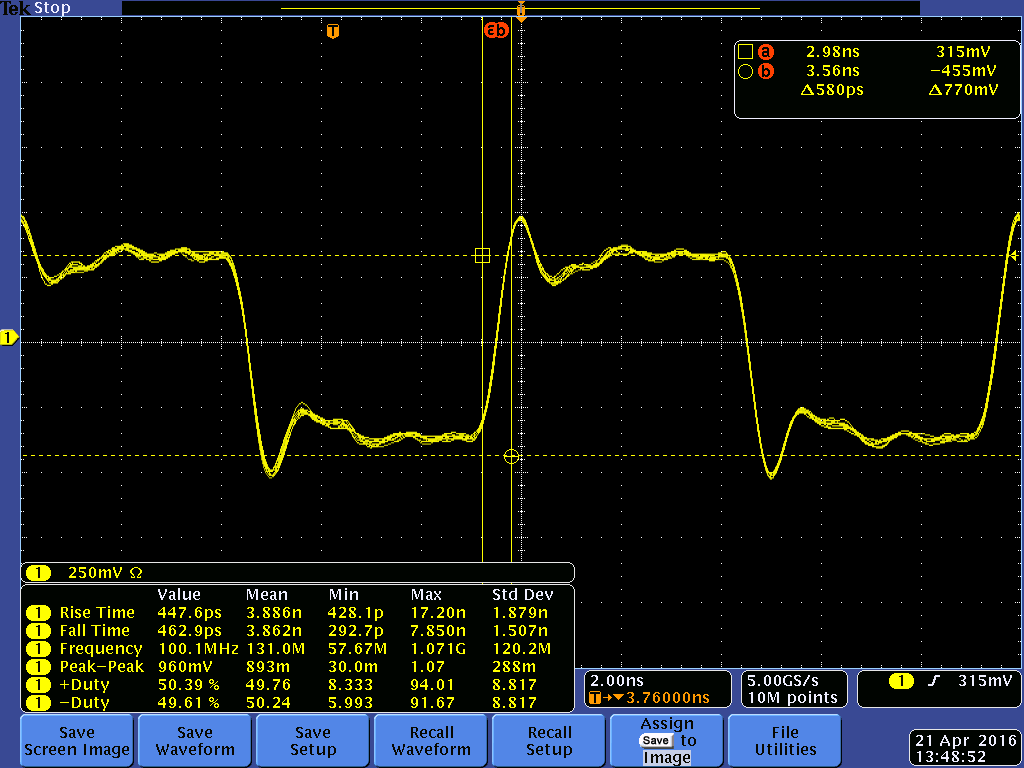
\includegraphics[scale = 0.2]{../img/stubs_oppsett_100mhz.png}}{\caption{$100~\mega\hertz$ measured using stubs.}\label{fig:measdiff2}}
   \end{floatrow}
\end{figure}

As shown in figure \ref{fig:measdiff2}, reflections still occurs. By doing the same measurements again with both the GPIO-card and the \gls{hdmi}-daughter card on both available \glspl{fpga}, the reflections remained somewhat the same. It is concluded that the most notable signal reflections is caused by the measurement setup, and will not affect the digital data when transmitting or receiving signals. This lead to the loop-back test using SignalTap II in an attempt to sample the signals (see chapter \ref{chap:sertest}).

\chapter{Testing and Verification of the Serial Interface} \label{chap:sertest}

\section{Hardware Simulation using Testbench in Modelsim}

\textit{To verify that the hardware design was working properly in terms of correct signal timing between the baudrate, \acrshort{uart} and decoder, a testbench was developed. The testbench was made using the \textit{Bitvis Utility Library} and the design simulation was done using Altera's Modelsim.}

\subsection{Purpose of Tests}

\begin{itemize}\setlength{\itemsep}{10pt}
\item Verify correct timing between the baudrate generator, clock and uart.
\item Verify correct timing for the uart decoder.
\item Verify that the design is working correctly in simulation.
\end{itemize}

\subsection{Experimental Setup}
\subsubsection{Bitvis Utility Library}
The \textit{Bitvis Utility Library} by Bitvis is an open source VHDL testbench infrastructure library for verification of FPGAs and ASICs \cite{bitvis16}. It was developed with the aim of simplifying the testbench development process when testing \acrshort{vhdl} designs. It was chosen for this test because of the ease of use and fast implementation (see uart\_tb.vhd for testbench implementation).\\

The main test procedure goes as follows: Send a request byte to the rx-signal, followed by a register-address. The request can be a read-request (0xDD) or a write-request (0xEE for '1' and 0xFF for '0'), and the address must be between 0x00 - 0xC1. Then, the tx-signal are sampled and compared with the requested address byte and checked for equality. If it is not equal, the test goes to a halt with a corresponding fault-message. The \textit{UART\_WRITE\_BYTE} and \textit{UART\_READ\_BYTE} testbench procedures were written with the main test procedure in mind. To simulate an incoming byte at the receiver, \textit{UART\_WRITE\_BYTE} inputs a vector of 8 bits as the data-byte. With the period of a transmitted bit, which is equal to $1/baud rate$, it outputs first a start bit, then the data bits and finally the stop bit. The rx-line takes the output of \textit{UART\_WRITE\_BYTE} as input. \textit{UART\_READ\_BYTE} takes the tx-line as input, and with the period of a transmitted bit shifts the tx-value into a data vector. Using the Bitvis \textit{check\_value}-function, the data vector is then checked and compared with the address-byte previously sent to the receiver. The \textit{UART\_READ\_BYTE} procedure is executed after the \textit{UART\_WRITE\_BYTE} procedure. \\

Other test procedures involves checking the constants found in \textit{uart\_gbt\_pkg.vhd} up against legal values, and also make sure that the tx- and rx-lines are in an idle state at the start of the test, i.e high bit value.

\subsection{Results}

\section{Connection between COM port and UART using SignalTap II}

\textit{By using SignalTap II to tap the transmitter and receiver lines, it is possible to verify that the \gls{fpga} design is responding correctly to the bytes sent from the C-program on the \gls{pc} side.} 

\subsection{Purpose of Tests}
\begin{itemize}\setlength{\itemsep}{10pt}
\item Verify that the C-program is in control of the \gls{com}.
\item Verify that there is communication between the \gls{fpga} \gls{uart} and the \gls{pc} \gls{com}.
\item Confirm that the \gls{fpga} design and C-program is working together the way they should.
\end{itemize}

\subsection{Experimental Setup}

\subsection{Results}

While testing the \gls{fpga} design, it occured that the \gls{uart} would hang after a random period of time. The reason as to why this was happening has yet to be found. A quick fix to this, however, was to simply implement a timer that would reset the \gls{uart} on the condition that no bytes have arrived in a given amount of time when the \gls{uart} is in the idle state. This is not a permanent fix, since there is a chance that the \gls{uart} might reset while a byte is under transmission. This might give an explanation as to why the C-program in some cases did not receive all the data it requested during transmission.

\section{Conclusion and Discussions}

\chapter{Conclusion and Discussion}

\end{document}